%package list
\documentclass{article}
\usepackage[top=3cm, bottom=3cm, outer=3cm, inner=3cm]{geometry}
\usepackage{multicol}
\usepackage{graphicx}
\usepackage{url}
%\usepackage{cite}
\usepackage{hyperref}
\usepackage{array}
%\usepackage{multicol}
\newcolumntype{x}[1]{>{\centering\arraybackslash\hspace{0pt}}p{#1}}
\usepackage{natbib}
\usepackage{pdfpages}
\usepackage{multirow}    
\usepackage[normalem]{ulem}
\useunder{\uline}{\ul}{}
\usepackage{svg}
\usepackage{xcolor}
\usepackage{listings}
\lstdefinestyle{ascii-tree}{
    literate={├}{|}1 {─}{--}1 {└}{+}1 
  }

\lstset{basicstyle=\ttfamily,
  showstringspaces=false,
  commentstyle=\color{red},
  keywordstyle=\color{blue}
}
%\usepackage{booktabs}
\usepackage{caption}
\usepackage{subcaption}
\usepackage{float}
\usepackage{array}

\usepackage{enumitem}


\newcolumntype{M}[1]{>{\centering\arraybackslash}m{#1}}
\newcolumntype{N}{@{}m{0pt}@{}}


%%%%%%%%%%%%%%%%%%%%%%%%%%%%%%%%%%%%%%%%%%%%%%%%%%%%%%%%%%%%%%%%%%%%%%%%%%%%
%%%%%%%%%%%%%%%%%%%%%%%%%%%%%%%%%%%%%%%%%%%%%%%%%%%%%%%%%%%%%%%%%%%%%%%%%%%%
\newcommand{\itemEmail}{vmaldonadov@unsa.edu.pe}
\newcommand{\itemStudent}{Victor Gonzalo Maldonado Vilca}
\newcommand{\itemCourse}{Programación Web 2}
\newcommand{\itemCourseCode}{1702122}
\newcommand{\itemSemester}{III}
\newcommand{\itemUniversity}{Universidad Nacional de San Agustín de Arequipa}
\newcommand{\itemFaculty}{Facultad de Ingeniería de Producción y Servicios}
\newcommand{\itemDepartment}{Departamento Académico de Ingeniería de Sistemas e Informática}
\newcommand{\itemSchool}{Escuela Profesional de Ingeniería de Sistemas}
\newcommand{\itemAcademic}{2024 - A}
\newcommand{\itemInput}{Del 9 de abril de 2024}
\newcommand{\itemOutput}{Al 29 de mayo de 2024}
\newcommand{\itemPracticeNumber}{06}
\newcommand{\itemTheme}{Django}
%%%%%%%%%%%%%%%%%%%%%%%%%%%%%%%%%%%%%%%%%%%%%%%%%%%%%%%%%%%%%%%%%%%%%%%%%%%%
%%%%%%%%%%%%%%%%%%%%%%%%%%%%%%%%%%%%%%%%%%%%%%%%%%%%%%%%%%%%%%%%%%%%%%%%%%%%

\usepackage[english,spanish]{babel}
\usepackage[utf8]{inputenc}
\AtBeginDocument{\selectlanguage{spanish}}
\renewcommand{\figurename}{Figura}
\renewcommand{\refname}{Referencias}
\renewcommand{\tablename}{Tabla} %esto no funciona cuando se usa babel
\AtBeginDocument{%
	\renewcommand\tablename{Tabla}
}

\usepackage{fancyhdr}
\pagestyle{fancy}
\fancyhf{}
\setlength{\headheight}{30pt}
\renewcommand{\headrulewidth}{1pt}
\renewcommand{\footrulewidth}{1pt}
\fancyhead[L]{\raisebox{-0.2\height}{
\includegraphics[width=3cm]{img/logo_episunsa.png}}}
\fancyhead[C]{\fontsize{7}{7}\selectfont	\itemUniversity \\ \itemFaculty \\ \itemDepartment \\ \itemSchool \\ \textbf{\itemCourse}}
\fancyhead[R]{\raisebox{-0.2\height}{
\includegraphics[width=1.2cm]{img/logo_abet}}}
\fancyfoot[L]{Victor M.}
\fancyfoot[C]{\itemCourse}
\fancyfoot[R]{Página \thepage}

% para el codigo fuente
\usepackage{listings}
\usepackage{color, colortbl}
\definecolor{dkgreen}{rgb}{0,0.6,0}
\definecolor{gray}{rgb}{0.5,0.5,0.5}
\definecolor{mauve}{rgb}{0.58,0,0.82}
\definecolor{codebackground}{rgb}{0.95, 0.95, 0.92}
\definecolor{tablebackground}{rgb}{0.8, 0, 0}

\lstset{frame=tb,
	language=bash,
	aboveskip=3mm,
	belowskip=3mm,
	showstringspaces=false,
	columns=flexible,
	basicstyle={\small\ttfamily},
	numbers=none,
	numberstyle=\tiny\color{gray},
	keywordstyle=\color{blue},
	commentstyle=\color{dkgreen},
	stringstyle=\color{mauve},
	breaklines=true,
	breakatwhitespace=true,
	tabsize=3,
	backgroundcolor= \color{codebackground},
}

\begin{document}
	
	\vspace*{10px}
	
	\begin{center}	
		\fontsize{17}{17} \textbf{ Informe de Laboratorio 06}
	\end{center}
	\centerline{\textbf{\Large Tema: \itemTheme}}
	%\vspace*{0.5cm}	

	\begin{flushright}
		\begin{tabular}{|M{2.5cm}|N|}
			\hline 
			\rowcolor{tablebackground}
			\color{white} \textbf{Nota}  \\
			\hline 
			     \\[30pt]
			\hline 			
		\end{tabular}
	\end{flushright}	

	\begin{table}[H]
		\begin{tabular}{|x{4.7cm}|x{4.8cm}|x{4.8cm}|}
			\hline 
			\rowcolor{tablebackground}
			\color{white} \textbf{Estudiante} & \color{white}\textbf{Escuela}  & \color{white}\textbf{Asignatura}   \\
			\hline 
			{\itemStudent \par \itemEmail} & \itemSchool & {\itemCourse \par Semestre: \itemSemester \par Código: \itemCourseCode}     \\
			\hline 			
		\end{tabular}
	\end{table}		
	
	\begin{table}[H]
		\begin{tabular}{|x{4.7cm}|x{4.8cm}|x{4.8cm}|}
			\hline 
			\rowcolor{tablebackground}
			\color{white}\textbf{Tarea} & \color{white}\textbf{Tema}  & \color{white}\textbf{Duración}   \\
			\hline 
			\itemPracticeNumber & \itemTheme & 2 horas   \\
			\hline 
		\end{tabular}
	\end{table}
	
	\begin{table}[H]
		\begin{tabular}{|x{4.7cm}|x{4.8cm}|x{4.8cm}|}
			\hline 
			\rowcolor{tablebackground}
			\color{white}\textbf{Semestre académico} & \color{white}\textbf{Fecha de inicio}  & \color{white}\textbf{Fecha de entrega}   \\
			\hline 
			\itemAcademic & \itemInput &  \itemOutput  \\
			\hline 
		\end{tabular}
	\end{table}
%%%%%%%%%%%%%%%%%%%%

  \section{Introducción}
  Django es un framework de desarrollo web en Python que facilita la creación rápida de aplicaciones web seguras y escalables.
  Ofrece un conjunto de herramientas integradas como ORM, administrador de Django y enrutamiento de URLs, lo que simplifica el 
  desarrollo y mejora la seguridad de las aplicaciones web.

%%%%%%%%%%%%%%%%%%%%

  \section{Objetivos}
  \begin{itemize}
    \item Entender y configurar el entorno de trabajo para Django
    \item Crear un primer proyecto en Django
    \item Crear apps e integrarlas al framework
  \end{itemize}

%%%%%%%%%%%%%%%%%%%%
 
	\section{Tarea}
  Implementa un Sistema en Django que maneje una tabla de Alumnos, una de Cursos y una de NotasAlumnosPorCurso y que 
  permita ingresar a nuevos alumnos, nuevos cursos y finalmente permita ingresar las notas por curso.
  \newpage
 
%%%%%%%%%%%%%%%%%%%% 
 
  \section{Entregables}
  \begin{itemize}
    \item Informe en Latex
    \item URL: Repositorio GitHub
    \item Link del vÍdeo (Youtube)
  \end{itemize}
  
%%%%%%%%%%%%%%%%%%%%    
		
	\section{Equipos, materiales y temas utilizados}
  \begin{itemize}
    \item Python
    \item Pip
    \item Django
    \item Entornos virtuales en python
    \item Proyectos de Django
    \item Aplicaciones en Django
    \item Modelos, Vistas, Templates y Formularios en Django
  \end{itemize}
 
%%%%%%%%%%%%%%%%%%%%

  \section{URL de Repositorio Github}
  \begin{itemize}
    \item URL del Repositorio GitHub
    \item \url{https://github.com/Victor-Gonzalo-Maldonado-Vilca/Lab06_Django.git}
  \end{itemize}
  
%%%%%%%%%%%%%%%%%%%%

	\section{Link de Video}
  \begin{itemize}
    \item Link del Vídeo Explicativo
    \item \url{https://www.youtube.com/watch?v=unhmxDkoSDY}
  \end{itemize}

%%%%%%%%%%%%%%%%%%%%

  \section{Metodología}

%%%%%%%%%%%%

  \subsection{Creación del entorno de Trabajo}
  
%%%%%%

  \subsubsection{Carpeta de trabajo}
  \begin{lstlisting}[language=, caption={Creación del Directorio}]
  mkdir lab06 && cd lab06
  \end{lstlisting}
  
%%%%%%

  \subsubsection{Creación del Entorno Virtual}
  \begin{lstlisting}[language=, caption={Creación Entorno virtual}]
  virtualenv -p python3 .
  \end{lstlisting}
  \newpage
  
%%%%%%%

  \subsubsection{Activar entorno Virtual}
  \begin{lstlisting}[language=, caption={Activar Entorno Virtual}]
  Scripts/activate
  \end{lstlisting}
  
%%%%%%

  \subsubsection{Instalar Django en el entorno Virtual}
  \begin{lstlisting}[language=, caption={Instalar Django}]
  pip install Django
  \end{lstlisting}
  
%%%%%%

  \subsubsection{Creación carpeta del proyecto}
  \begin{lstlisting}[language=, caption={Carpeta src}]
  mkdir src && cd src
  \end{lstlisting}
  
%%%%%%

  \subsubsection{Inicializar git}
  \begin{lstlisting}[language=, caption={Inicializar git}]
  git init
  \end{lstlisting}
  
%%%%%%

  \subsubsection{Crear .gitignore}
  Seguimos el siguiente Repositorio \url{https://github.com/django/django/blob/main/.gitignore}
  
%%%%%%%%%%%%
  
  \subsection{Creacion del proyecto y apps}
  
%%%%%%

  \subsubsection{Crear Proyecto}
  \begin{lstlisting}[language=, caption={Crear proyecto}]
  django-admin startproject mi_proyecto
  \end{lstlisting}
  
%%%%%%

  \subsubsection{Crear App}
  \begin{lstlisting}[language=, caption={Crear App}]
  python manage.py startapp gestion_Universitario
  \end{lstlisting}
  \newpage
  
%%%%%%%%%%%%%%%%%%%%

  \section{Desarrollo del trabajo}
  
%%%%%%%%%%%%

  \subsection{Configuramos el proyecto en settings.py}
  
%%%%%%

  \subsubsection{Cambiamos el idioma y zona del tiempo}
  \begin{figure}[H]
    \centering
    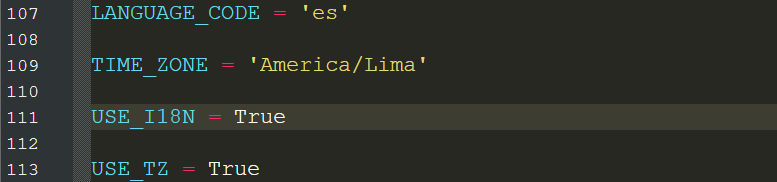
\includegraphics[width=1\textwidth, keepaspectratio]{img/lenguaje.png}
    \caption{Configuración a nuestra región}
  \end{figure}

%%%%%%

  \subsubsection{Agregamos la aplicación en el archivo settings.py}
  \begin{figure}[H]
    \centering
    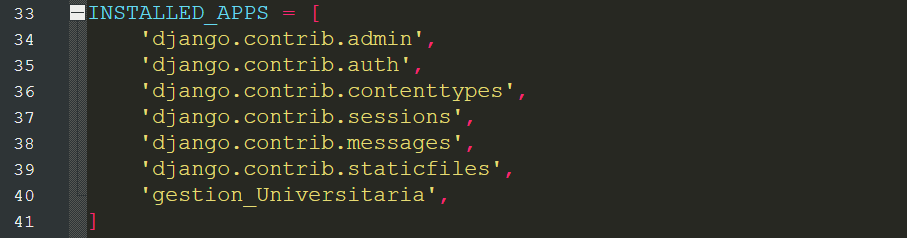
\includegraphics[width=1\textwidth, keepaspectratio]{img/app.png}
    \caption{Agregar App}
  \end{figure}
  
%%%%%%%%%%%%

  \subsection{Definir Modelos en models.py en la App gestionUniversitaria}
  
%%%%%%

  \subsubsection{Modelo de Alumno}
  Esta parte del código define un modelo de Django llamado Alumno con campos como CUI, nombre, apellidos, edad y DNI, 
  cada uno con validaciones específicas para garantizar la integridad de los datos. El método str devuelve una representación 
  legible del objeto Alumno, concatenando el nombre y apellidos del alumno.
  \begin{lstlisting}[language=python, caption={Modelo Alumno}]
  class Alumno(models.Model):
    cui = models.IntegerField(
      validators=[
        MinValueValidator(10000000, message="Se requiere 8 digitos"), 
        MaxValueValidator(99999999, message="Se requiere 8 digitos")
      ], 
      unique=True
    )
    nombre = models.CharField(max_length=100)
    apellidos = models.CharField(max_length=100)
    edad = models.IntegerField(validators=[MinValueValidator(0), MaxValueValidator(100)])
    dni = models.IntegerField(
      validators=[
        MinValueValidator(10000000, message="Se requiere 8 digitos"), 
        MaxValueValidator(99999999, message="Se requiere 8 digitos")
      ]
    )
    
    def __str__(self):
      return f"{self.nombre} {self.apellidos}"
  \end{lstlisting}
  
%%%%%%

  \subsubsection{Modelo de Curso}
  Esta parte del código está diseñado para manejar información sobre cursos universitarios, incluyendo su identificación única, 
  nombre y cualquier otra información relacionada que pueda añadirse en futuras modificaciones del modelo.
  \begin{lstlisting}[language=python, caption={Modelo Curso}]
  class Curso(models.Model):
    codigo = models.IntegerField(
      validators=[
        MinValueValidator(1000000, message="Se requiere 7 digitos"), 
        MaxValueValidator(9999999, message="Se requiere 7 digitos")
      ]
    )
    nombre = models.CharField(max_length=100)
    
    def __str__(self):
      return self.nombre
  \end{lstlisting}

%%%%%%

  \subsubsection{Modelo de NotasAlumnosPorCurso}
  El modelo NotasAlumnosPorCurso en Django almacena las notas de los alumnos por curso, relacionando cada 
  registro con un alumno y un curso específicos. Utiliza un campo decimal para representar las notas con precisión de 2 decimales.
  \begin{lstlisting}[language=python, caption={Modelo NotasAlumnosPorCurso}]
  class NotasAlumnosPorCurso(models.Model):
    alumno = models.ForeignKey(Alumno, on_delete=models.CASCADE)
    curso = models.ForeignKey(Curso, on_delete=models.CASCADE)
    notas = models.DecimalField(max_digits=5, decimal_places=2)
    
    def __str__(self):
      return f"La nota del Alumno: {self.alumno.nombre} {self.alumno.apellidos}, es = {self.notas}"
  \end{lstlisting}
  \newpage
  
%%%%%%%%%%%%

  \subsection{Crear y Aplicar Migraciones}
  \begin{lstlisting}[language=, caption={Crear Migraciones}]
  python manage.py makemigrations gestion_Universitaria
  \end{lstlisting}
  \begin{lstlisting}[language=, caption={Aplicar Migraciones}]
  python manage.py migrate
  \end{lstlisting}
  
%%%%%%%%%%%%

  \subsection{Crear Formularios}
  \textit{Nos encontramos en forms.py de la aplicación gestionUniversitaria}
  
%%%%%%

  \subsubsection{Formulario AlumnoForm}
  Formulario asociado al modelo Alumno, permite ingresar información sobre un alumno como CUI, nombre, apellidos, edad y DNI.
  \begin{lstlisting}[language=python, caption={Formulario AlumnoForm}]
  class AlumnoForm(forms.ModelForm):
  
    class Meta:
      model = Alumno
      fields = ['cui', 'nombre', 'apellidos', 'edad', 'dni']
  \end{lstlisting}
  
%%%%%%

  \subsubsection{Formulario CursoForm}
  Formulario asociado al modelo Curso, utilizado para ingresar información sobre un curso como código y nombre.
  \begin{lstlisting}[language=python, caption={Formulario CursoForm}]
  class CursoForm(forms.ModelForm):

    class Meta:
      model = Curso
      fields = ['codigo', 'nombre']
  \end{lstlisting}
  
%%%%%%

  \subsubsection{Formulario NotasAlumnosPorCursoForm}
  Formulario vinculado al modelo NotasAlumnosPorCurso, permite registrar las notas de un alumno en un curso específico. 
  Incluye campos para seleccionar el alumno, el curso y la nota.
  \begin{lstlisting}[language=python, caption={Formulario NotasAlumnosPorCursoForm}]
  class NotasAlumnosPorCursoForm(forms.ModelForm):
    alumno = forms.ModelChoiceField(queryset=Alumno.objects.all(), label='Alumno')
    curso = forms.ModelChoiceField(queryset=Curso.objects.all(), label='Curso')
    
    class Meta:
      model = NotasAlumnosPorCurso
      fields = ['alumno', 'curso', 'notas']
  \end{lstlisting}
  \newpage
  
%%%%%%%%%%%%

  \subsection{Crear Vistas}
  \textit{Nos encontramos en views.py de la aplicación gestionUniversitaria}
  
%%%%%%

  \subsubsection{Vista agregarAlumno}
  Esta vista maneja la creación de un nuevo alumno. Si el método de la solicitud es POST, crea un formulario 
  AlumnoForm a partir de los datos de la solicitud y, si es válido, guarda el formulario y redirige a la misma 
  vista para mostrar el formulario vacío. Si el método de la solicitud no es POST, simplemente muestra un 
  formulario vacío para agregar un alumno y una lista de todos los alumnos existentes.
  \begin{lstlisting}[language=python, caption={Vista agregarAlumno}]
  def agregar_alumno(request):
    if request.method == 'POST':
      form = AlumnoForm(request.POST)
      if form.is_valid():
        form.save()
        return redirect('agregar_alumno')
    else:
      form = AlumnoForm()

    alumnos = Alumno.objects.all()
    return render(request, 'gestion_Universitaria/agregar_alumno.html', {'form': form, 'alumnos': alumnos})
  \end{lstlisting}
  
%%%%%%

  \subsubsection{Vista agregarCurso}
  Esta vista gestiona la creación de un nuevo curso. Similar a la vista agregarAlumno, crea un formulario CursoForm 
  a partir de los datos de la solicitud y, si es válido, guarda el formulario y redirige a la misma vista para mostrar 
  el formulario vacío. Si el método de la solicitud no es POST, simplemente muestra un formulario vacío para agregar 
  un curso y una lista de todos los cursos existentes.
  \begin{lstlisting}[language=python, caption={Vista agregarCurso}]
  def agregar_curso(request):
    if request.method == 'POST':
      form = CursoForm(request.POST)
      if form.is_valid():
        form.save()
        return redirect('agregar_curso')
    else:
      form = CursoForm()
      
    cursos = Curso.objects.all()
    return render(request, 'gestion_Universitaria/agregar_curso.html', {'form': form, 'cursos': cursos})
  \end{lstlisting}
  
%%%%%%
  
  \subsubsection{Vista agregarNotasAlumnosPorCurso}
  Esta vista maneja la creación de nuevas notas para los alumnos en un curso específico. Al igual que las vistas anteriores, 
  crea un formulario NotasAlumnosPorCursoForm a partir de los datos de la solicitud y, si es válido, guarda el formulario y 
  redirige a la misma vista para mostrar el formulario vacío. Si el método de la solicitud no es POST, simplemente muestra un 
  formulario vacío para agregar notas y una lista de todas las notas existentes.
  \begin{lstlisting}[language=python, caption={Vista agregarNotasAlumnosPorCurso}]
  def agregar_notas_alumnos_por_curso(request):
    if request.method == 'POST':
      form = NotasAlumnosPorCursoForm(request.POST)
      if form.is_valid():
        form.save()
        return redirect('agregar_nota')
    else:
      form = NotasAlumnosPorCursoForm()
      
    notas = NotasAlumnosPorCurso.objects.all()
    return render(request, 'gestion_Universitaria/agregar_nota.html', {'form': form, 'notas': notas})
  \end{lstlisting}
  
%%%%%%%%%%%%

  \subsection{Crear Plantillas}
  En esta parte se verán los HTML, no nos interesará fragmentos de código propios de este, sino las novedades de Django como bucles para 
  iterar todos los datos como los formularios para ingresar datos.
  
%%%%%%

  \subsubsection{Archivo HTML agregarAlumnos}
  \begin{itemize}
    \item \textbf{Descripción: }Este archivo HTML representa una página web enfocada en la administración de alumnos universitarios. 
    Está dividida en dos secciones clave:
    \newline
    En la primera sección, se presenta un formulario que permite añadir nuevos alumnos. Este formulario cuenta con medidas de 
    seguridad, como el token CSRF, y un botón "Guardar" para enviar la información al servidor. También incluye enlaces a otras 
    áreas del sistema, como la lista de alumnos, cursos y las notas de los alumnos.
    \newline
    La segunda parte de la página muestra una tabla que contiene los detalles de los alumnos ya registrados en la base de datos. 
    Si no hay alumnos registrados, se muestra un mensaje indicando esta ausencia. La tabla presenta información como el CUI, 
    nombres, apellidos, edad y DNI de cada alumno.
    \item \textbf{Código: }
    \begin{lstlisting}[language=html, caption={HTML agregarAlumnos}]
    <!DOCTYPE HTML>
    <html>
      <head>
        <title>Agregar Alumnos</title>
        <meta charset="UTF-8"/>
        <meta name="author" content="Victor Gonzalo Maldonado Vilca"/>
        <meta name="description" content="Agregar alumnos universitarios"/>
        <meta name="keywords" content="alumnos, agregar, universidad"/>
        <meta name="viewport" content="width=device-width, initial-scale=1.0"/>
      </head>
      <body>
        <div>
          <h1>Agregar Alumnos</h1>
          <form method="POST">
            
            {{ form.as_p }}
            <button type="submit">Guardar</button>
          </form>
          <a href="#">Lista de Alumnos</a>
          <a href="">Lista de Cursos</a>
          <a href="">Notas de los Alumnos</a>
        </div>
        <div>
          <h1>Lista de Alumnos</h1>
          
            <table border="1" style="text-align: center">
              <tr>
                <th>CUI</th>
                <th>Nombre</th>
                <th>Apellidos</th>
                <th>Edad</th>
                <th>DNI</th>
              </tr>
              
                <tr>
                  <td>{{ alumno.cui }}</td>
                  <td>{{ alumno.nombre }}</td>
                  <td>{{ alumno.apellidos }}</td>
                  <td>{{ alumno.edad }}</td>
                  <td>{{ alumno.dni }}</td>
                </tr>
              
            
            </table>
          
            <p>No hay alumnos en la base de datos.</p>
          
        </div>
      </body>
    </html>
    \end{lstlisting}
  \end{itemize}
  
%%%%%%

  \subsubsection{Archivo HTML agregarCursos}
  \begin{itemize}
    \item \textbf{Descripción: }Este código HTML representa una página web para la gestión de cursos universitarios. 
    Incluye un formulario para agregar cursos, con un campo para ingresar información sobre nuevos cursos, un botón Guardar 
    para enviar el formulario al servidor y enlaces a otras secciones del sistema. También muestra una lista de cursos 
    existentes en una tabla, mostrando el código y el nombre de cada curso si hay cursos registrados, o un mensaje indicando 
    la ausencia de cursos en caso contrario.
    \item \textbf{Código: }
    \begin{lstlisting}[language=html, caption={HTML agregarCursos}]
    <!DOCTYPE HTML>
    <html>
      <head>
        <title>Agregar Cursos</title>
        <meta charset="UTF-8"/>
        <meta name="author" content="Victor Gonzalo Maldonado Vilca"/>
        <meta name="description" content="Agregar cursos universitarios"/>
        <meta name="keywords" content="cursos, agregar, universidad"/>
        <meta name="viewport" content="width=device-width, initial-scale=1.0"/>
      </head>
      <body>
        <div>
          <h1>Agregar Cursos</h1>
          <form method="POST">
            
            {{ form.as_p }}
            <button type="submit">Guardar</button>
          </form>
          <a href="">Lista de Alumnos</a>
          <a href="#">Lista de Cursos</a>
          <a href="">Notas de los Alumnos</a>
        </div>
        <div>
          <h1>Lista de Cursos</h1>
          
            <table border="1" style="text-align: center">
              <tr>
                <th>Codigo</th>
                <th>Nombre del Curso</th>
              </tr>
              
                <tr>
                  <td>{{ curso.codigo }}</td>
                  <td>{{ curso.nombre }}</td>
                </tr>
              
            
            </table>
          
            <p>No hay cursos en la base de datos.</p>
          
        </div>
      </body>
    </html>
    \end{lstlisting}
    
  \end{itemize}
 
%%%%%%

  \subsubsection{Archivo HTML agregarNotas}
  \begin{itemize}
    \item \textbf{Descripción: }Este código HTML crea una página web para agregar y mostrar notas de alumnos en cursos universitarios. 
    Incluye un formulario para ingresar nuevas notas, enlaces a la lista de alumnos y cursos, y una tabla para mostrar las notas 
    existentes. La tabla presenta información como el nombre del alumno, el curso y las notas obtenidas. Si no hay notas 
    registradas, se muestra un mensaje indicando esta situación.
    \item \textbf{Código: }
    \begin{lstlisting}[language=html, caption={HTML agregarNotas}]
    <!DOCTYPE HTML>
    <html>
      <head>
        <title>Agregar Notas</title>
        <meta charset="UTF-8"/>
        <meta name="author" content="Victor Gonzalo Maldonado Vilca"/>
        <meta name="description" content="Agregar notas"/>
        <meta name="keywords" content="notas, agregar, universidad"/>
        <meta name="viewport" content="width=device-width, initial-scale=1.0"/>
      </head>
      <body>
        <div>
          <h1>Agregar Notas</h1>
          <form method="POST">
            
            {{ form.as_p }}
            <button type="submit">Guardar</button>
          </form>
          <a href="">Lista de Alumnos</a>
          <a href="">Lista de Cursos</a>
          <a href="#">Notas de los Alumnos</a>
        </div>
        <div>
          <h1>Lista de Alumnos - curso - nota</h1>
          
            <table border="1" style="text-align: center">
              <tr>
                <th>Alumno</th>
                <th>Curso</th>
                <th>Notas</th>
              </tr>
              
                <tr>
                  <td>{{ nota.alumno}}</td>
                  <td>{{ nota.curso }}</td>
                  <td>{{ nota.notas }}</td>
                </tr>
              
            
            </table>
          
            <p>No hay notas en la base de datos.</p>
          
        </div>
      </body>
    </html>
    \end{lstlisting}
   
  \end{itemize}
  
%%%%%%

  \subsubsection{CSS} 
  Los estilos usados son básicos simples cambios de color al igual que alineación de palabras, las clases y posiblemente id simplemente,
  se colocaron por buena práctiva.
  
%%%%%%%%%%%%

  \subsection{Configurar URLS}
  
%%%%%%

  \subsubsection{Configurar las URLs en urls.py de la aplicación gestionUniversitaria}
  \begin{itemize}
    \item \textbf{Descripción: }El archivo de configuración de urls en Django está diseñado para asignar rutas (URLs) a 
    tres vistas diferentes en una aplicación web. La primera ruta está vinculada a la vista agregarAlumno, la segunda a la vista 
    agregarCurso, y la tercera a la vista agregarNotasAlumnosPorCurso. Cuando un usuario accede a las URLs /alumnos/, /cursos/, 
    o /notas/, Django activa la función correspondiente para manejar la solicitud. Los nombres asignados (name) a cada ruta 
    facilitan su referencia en otras partes del código, como enlaces (links) dentro de los templates HTML.
    \item \textbf{Código: }
    \begin{lstlisting}[language=python, caption={urls.py de la App}]
    from django.urls import path
    from . import views

    urlpatterns = [
      path('alumnos/', views.agregar_alumno, name='agregar_alumno'),
      path('cursos/', views.agregar_curso, name='agregar_curso'),
      path('notas/', views.agregar_notas_alumnos_por_curso, name='agregar_nota'),
    ]
    \end{lstlisting}
  \end{itemize}
  
%%%%%%

  \subsubsection{Configurar las URLs en urls.py del proyecto}
  \begin{itemize}
    \item \textbf{Descripción: }En el fragmento de código Python del archivo de configuración de URLs (urls.py) 
    del proyecto Django, se importan las funciones necesarias para definir rutas de URL (path) y para incluir 
    otro archivo de configuración de URLs (include). Posteriormente, se establecen las URLs principales del proyecto: 
    la URL /admin/ se asigna a la interfaz de administración de Django, mientras que la URL raíz ('') se asigna a las URLs 
    definidas en el archivo urls.py de la aplicación gestionUniversitaria. Esta configuración implica que todas las URLs 
    que comiencen con la raíz del sitio, como /, /alumnos/, /cursos/, etc., serán gestionadas por las URLs definidas en 
    gestionUniversitaria.urls.
    \item \textbf{Código: }
    \begin{lstlisting}[language=python, caption={urls.py del proyecto}]
    from django.contrib import admin
    from django.urls import path, include

    urlpatterns = [
      path('admin/', admin.site.urls),
      path('', include('gestion_Universitaria.urls')),
    ]
    \end{lstlisting}
  \end{itemize}

%%%%%%

  \subsubsection{Ejecutar el Servidor}
  \begin{lstlisting}[language=, caption={Servidor}]
  python manage.py runserver
  \end{lstlisting}
  
%%%%%%
  
  \newpage
  \subsubsection{Ejecutando la Aplicación}
  \begin{itemize}
    \item Agregar Alumnos:
    \begin{figure}[H]
      \centering
      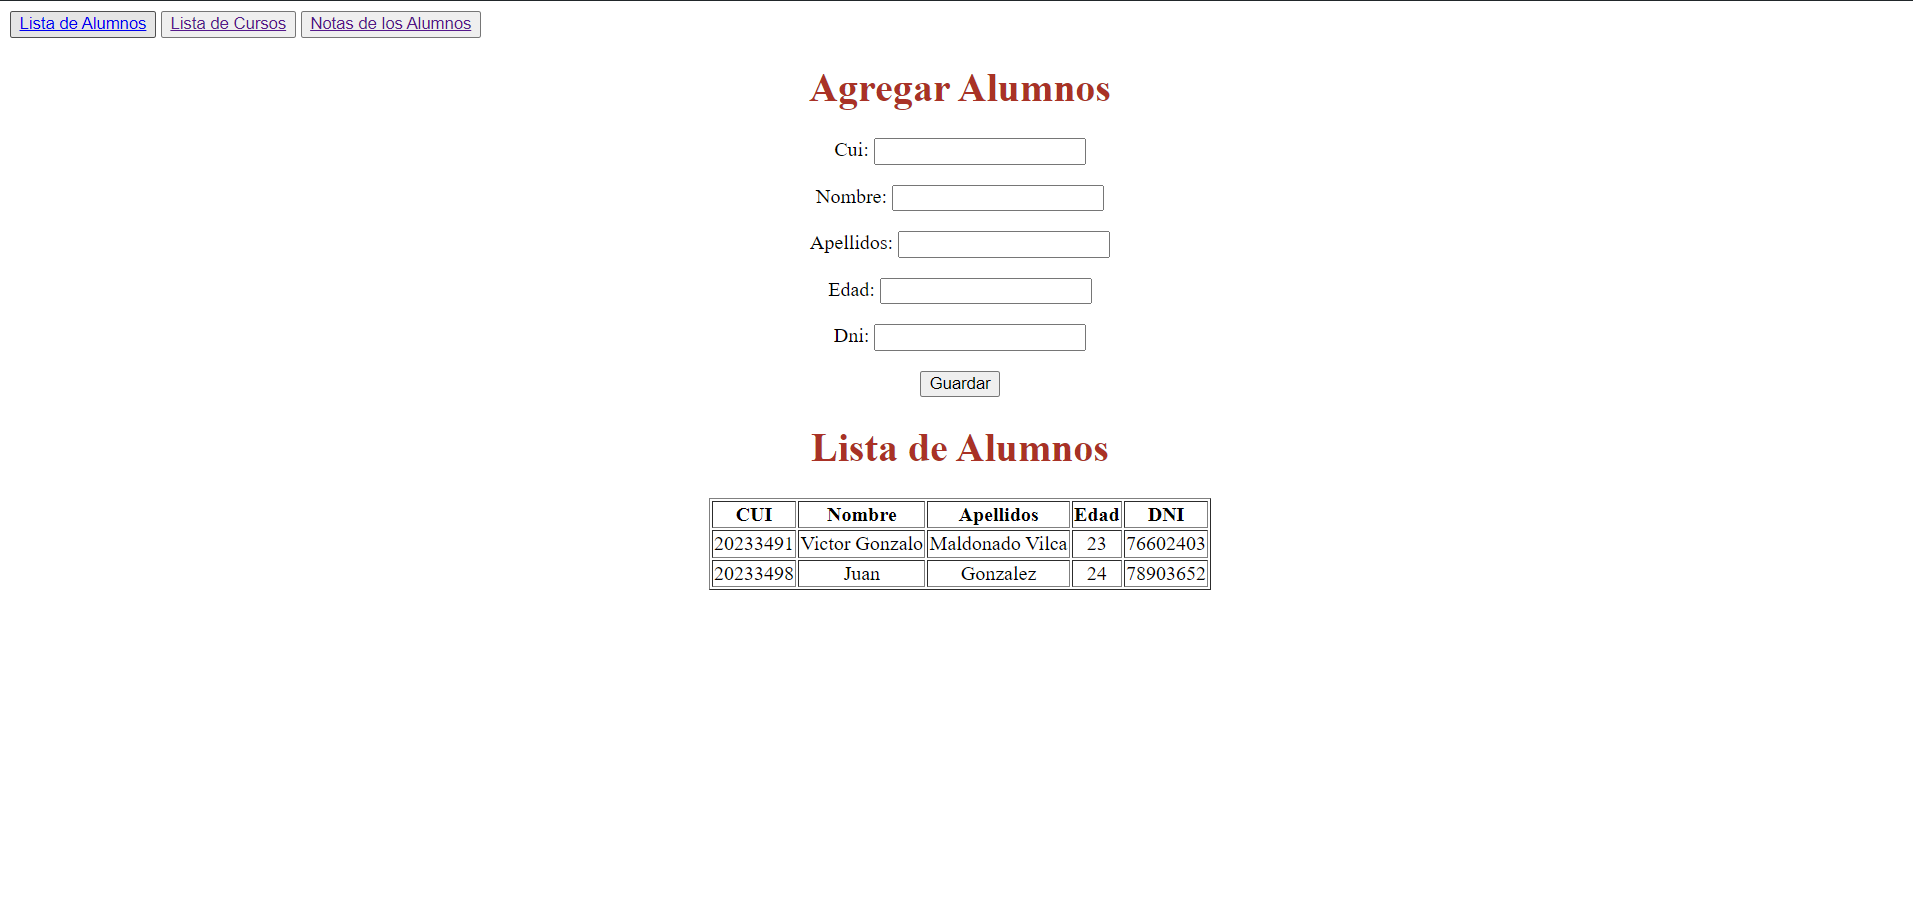
\includegraphics[width=1\textwidth, keepaspectratio]{img/html1.png}
      \caption{Agregar Alumnos}
    \end{figure}
    \begin{figure}[H]
      \centering
      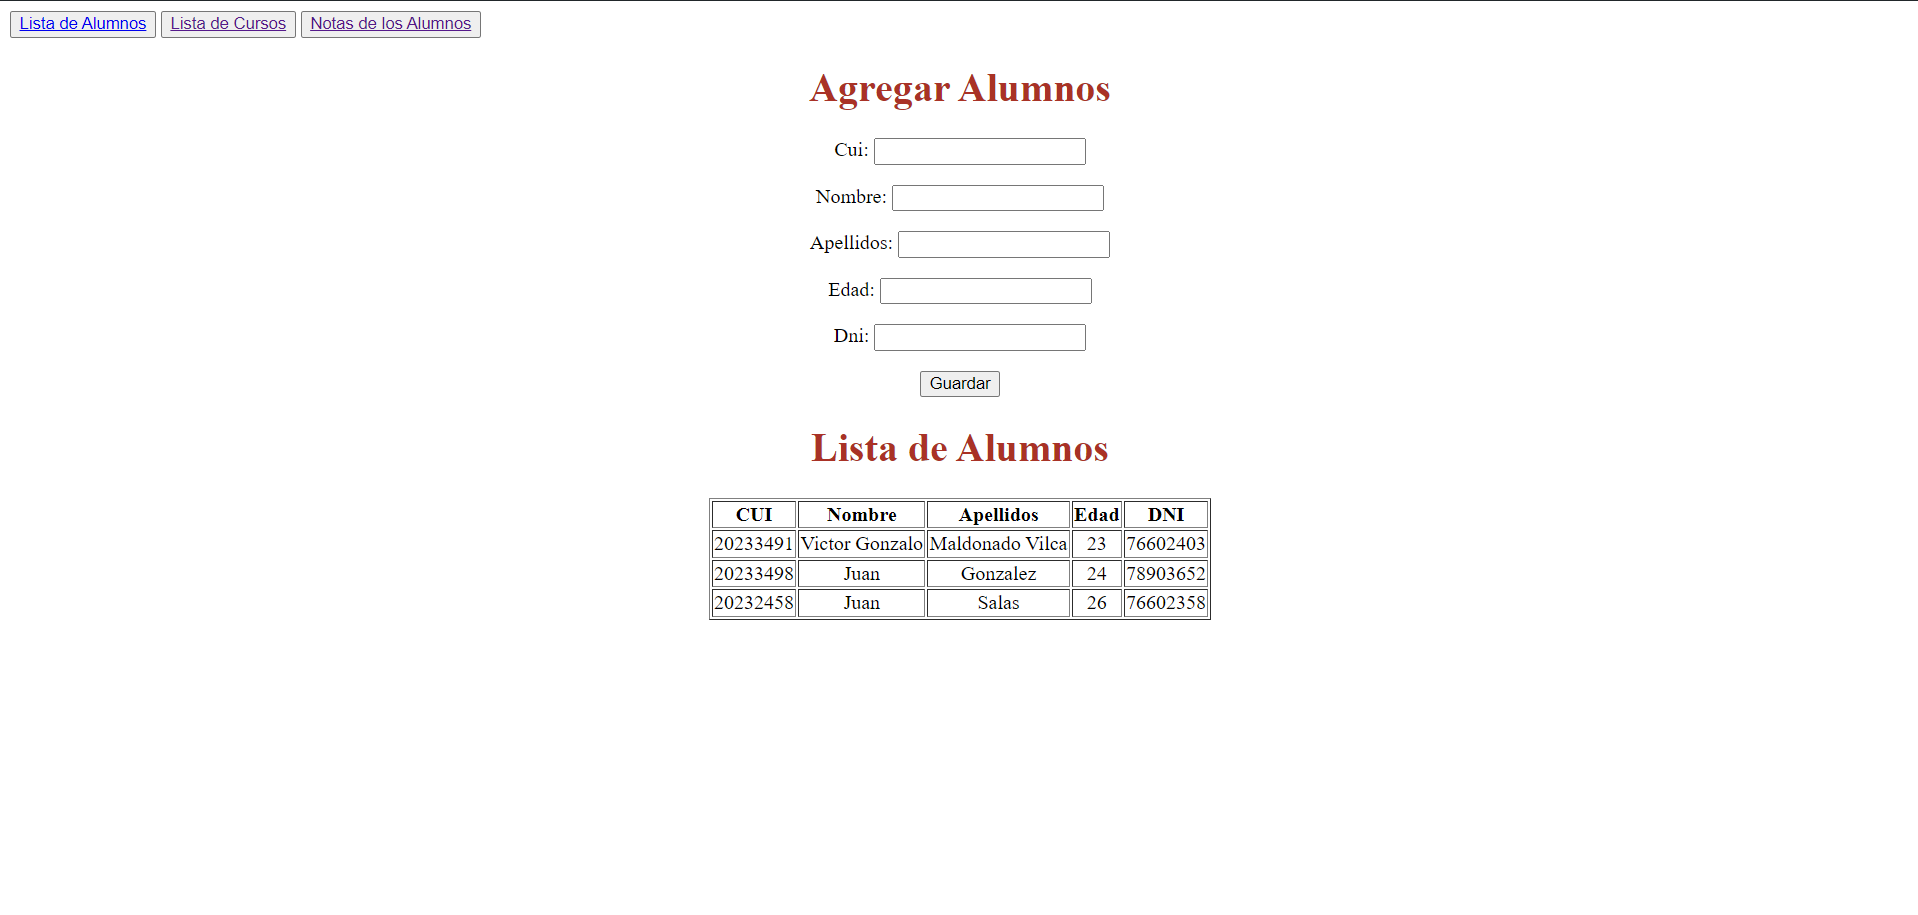
\includegraphics[width=1\textwidth, keepaspectratio]{img/html2.png}
      \caption{Agregar Alumnos}
    \end{figure}
    \newpage
    \item Agregar Cursos:
    \begin{figure}[H]
      \centering
      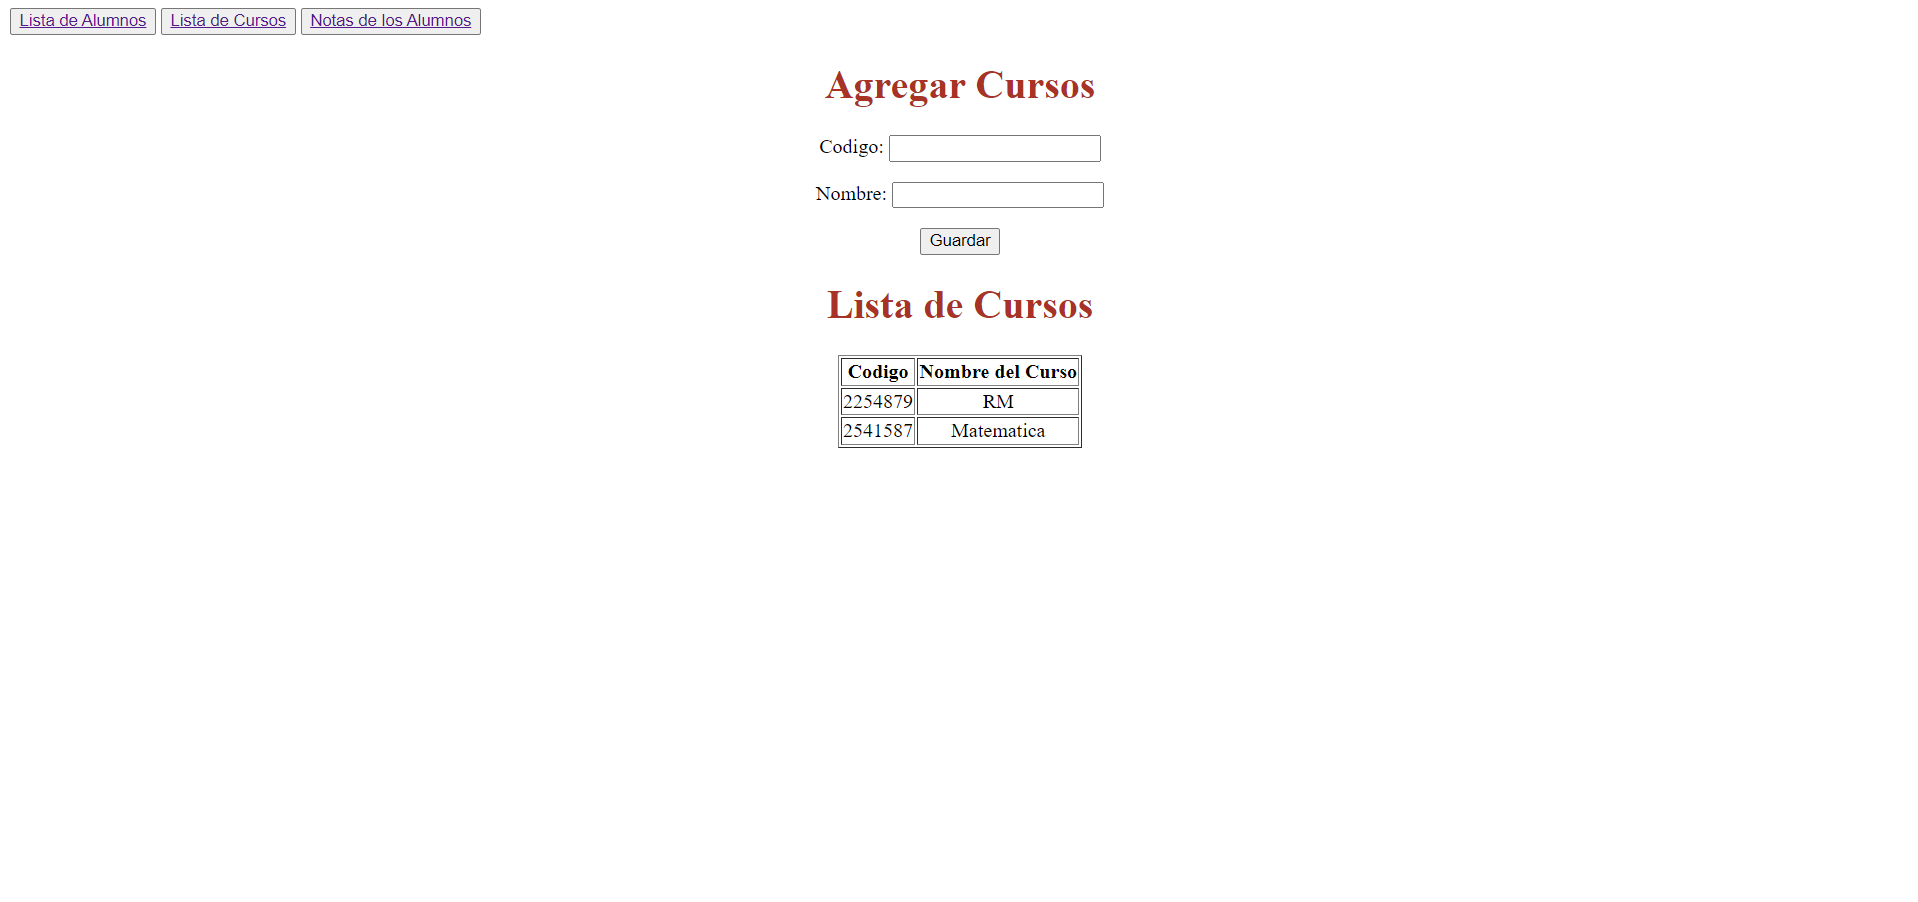
\includegraphics[width=1\textwidth, keepaspectratio]{img/html3.png}
      \caption{Agregar Cursos}
    \end{figure}
    \begin{figure}[H]
      \centering
      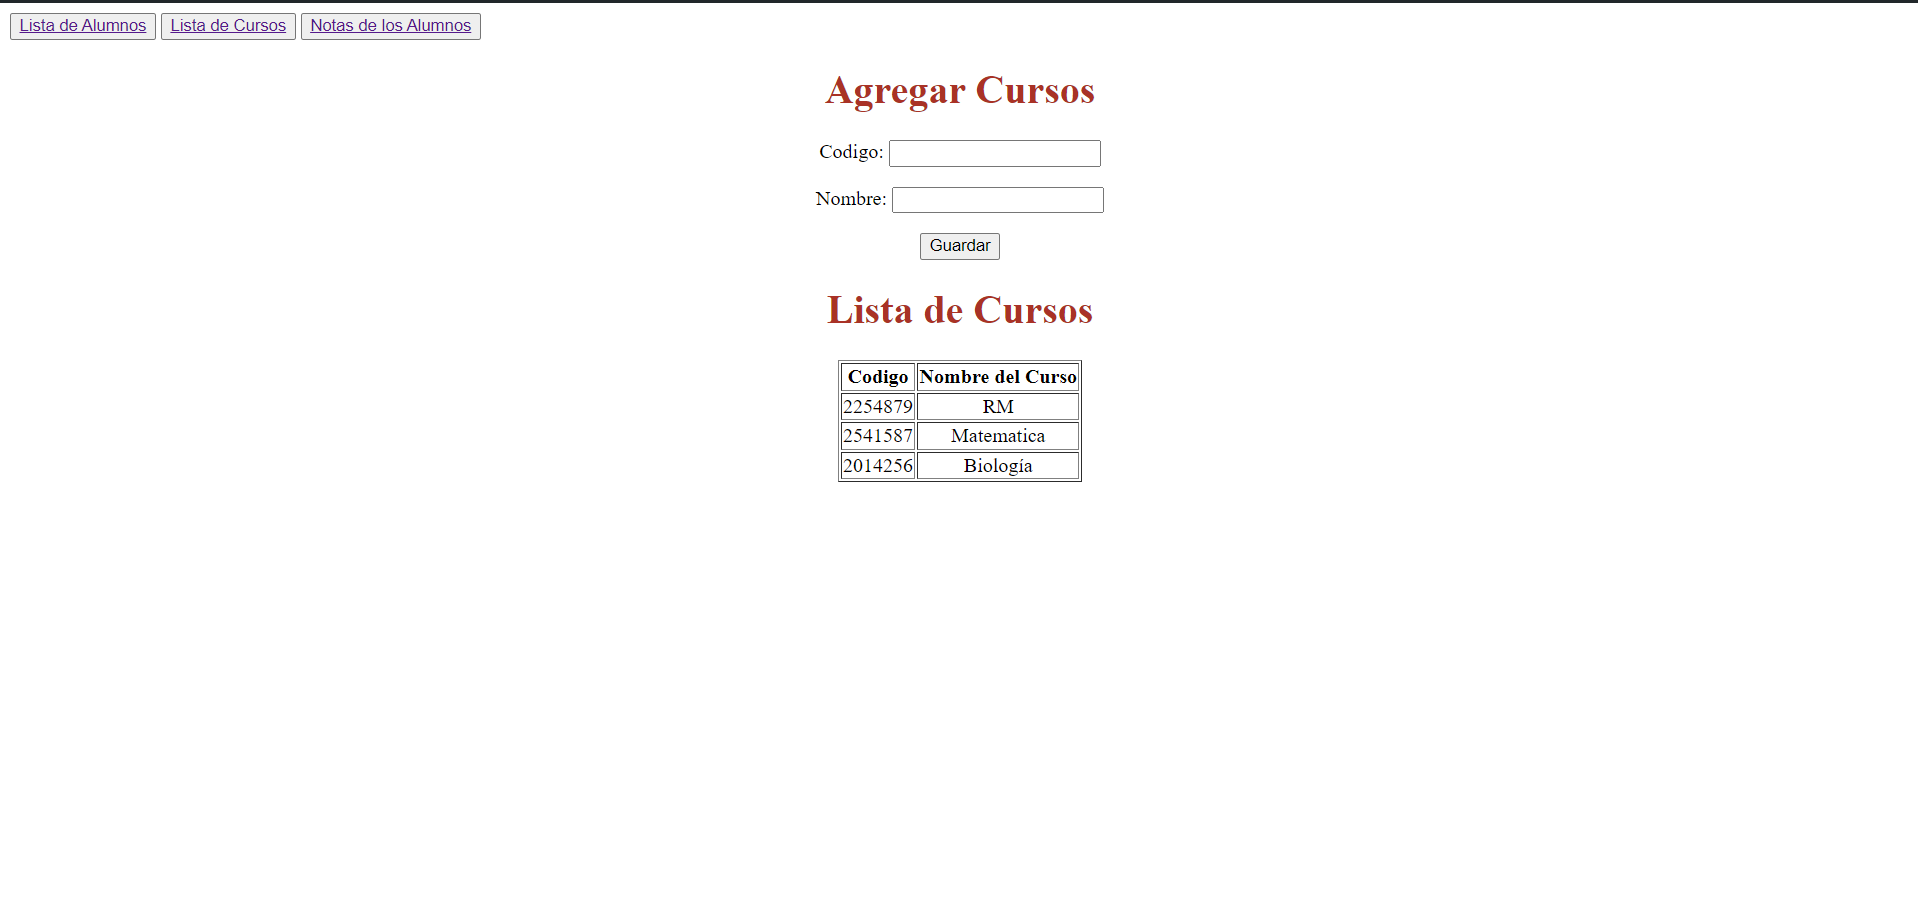
\includegraphics[width=1\textwidth, keepaspectratio]{img/html4.png}
      \caption{Agregar Cursos}
    \end{figure}
    \newpage
    \item Agregar Notas:
    \begin{figure}[H]
      \centering
      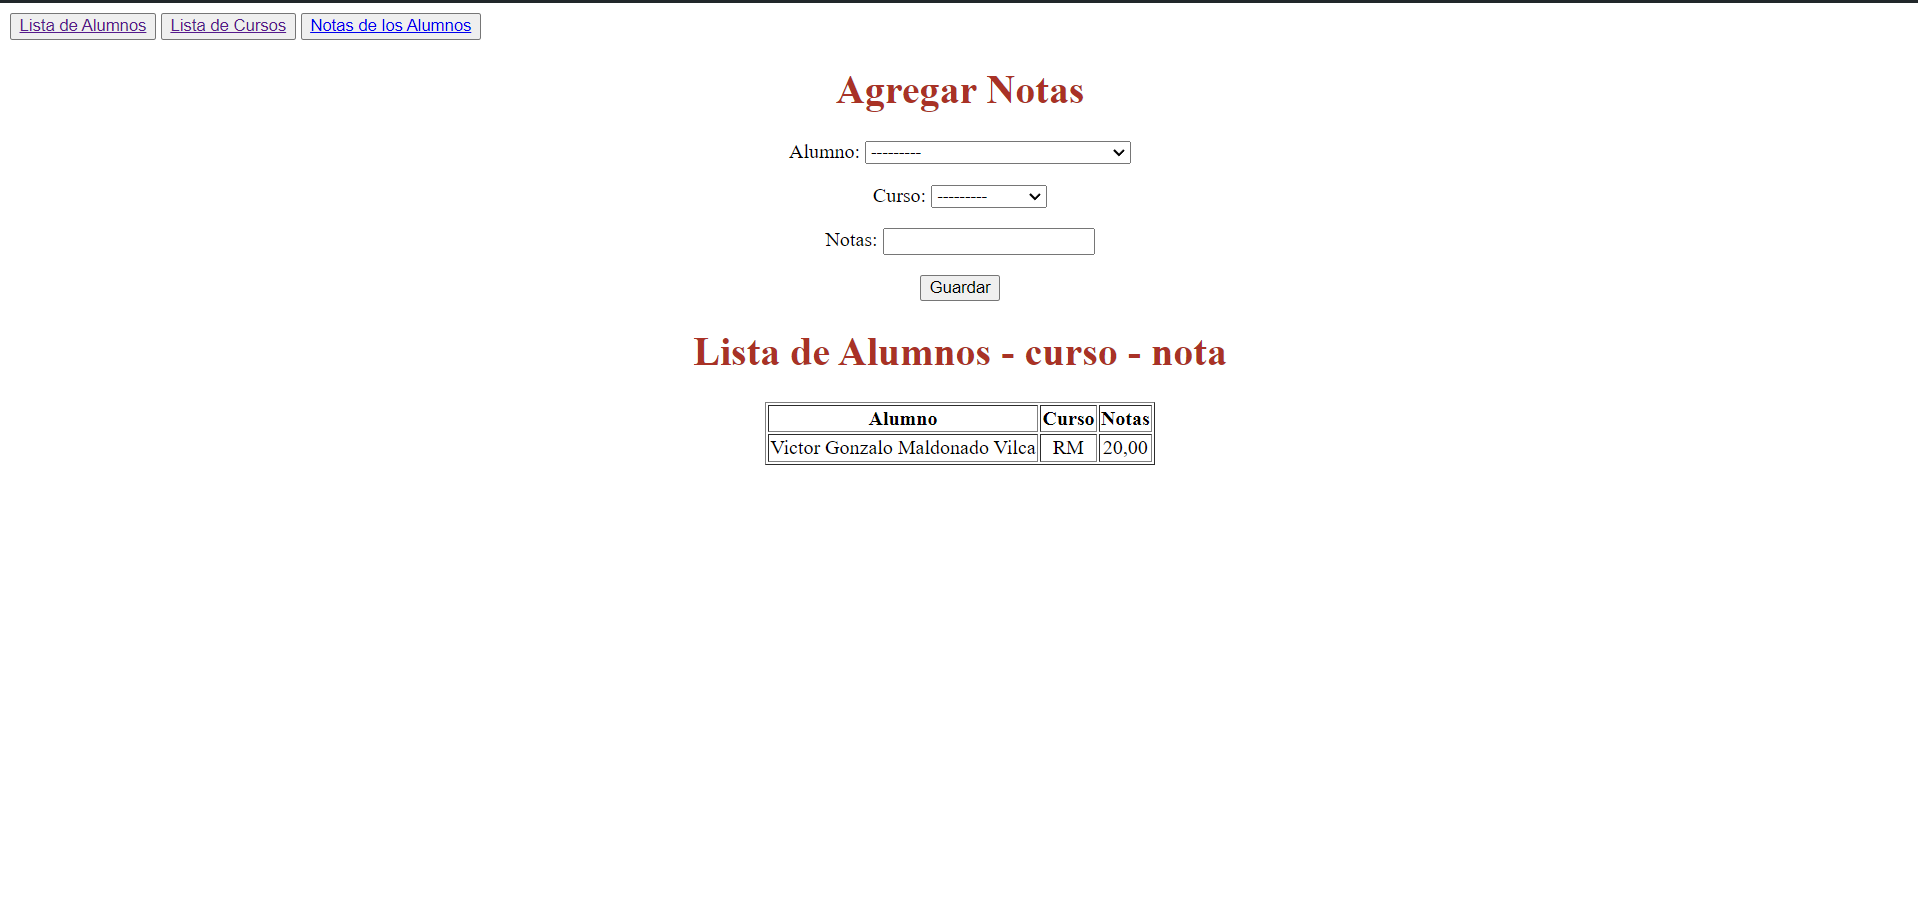
\includegraphics[width=1\textwidth, keepaspectratio]{img/html5.png}
      \caption{Agregar Notas}
    \end{figure}
    \begin{figure}[H]
      \centering
      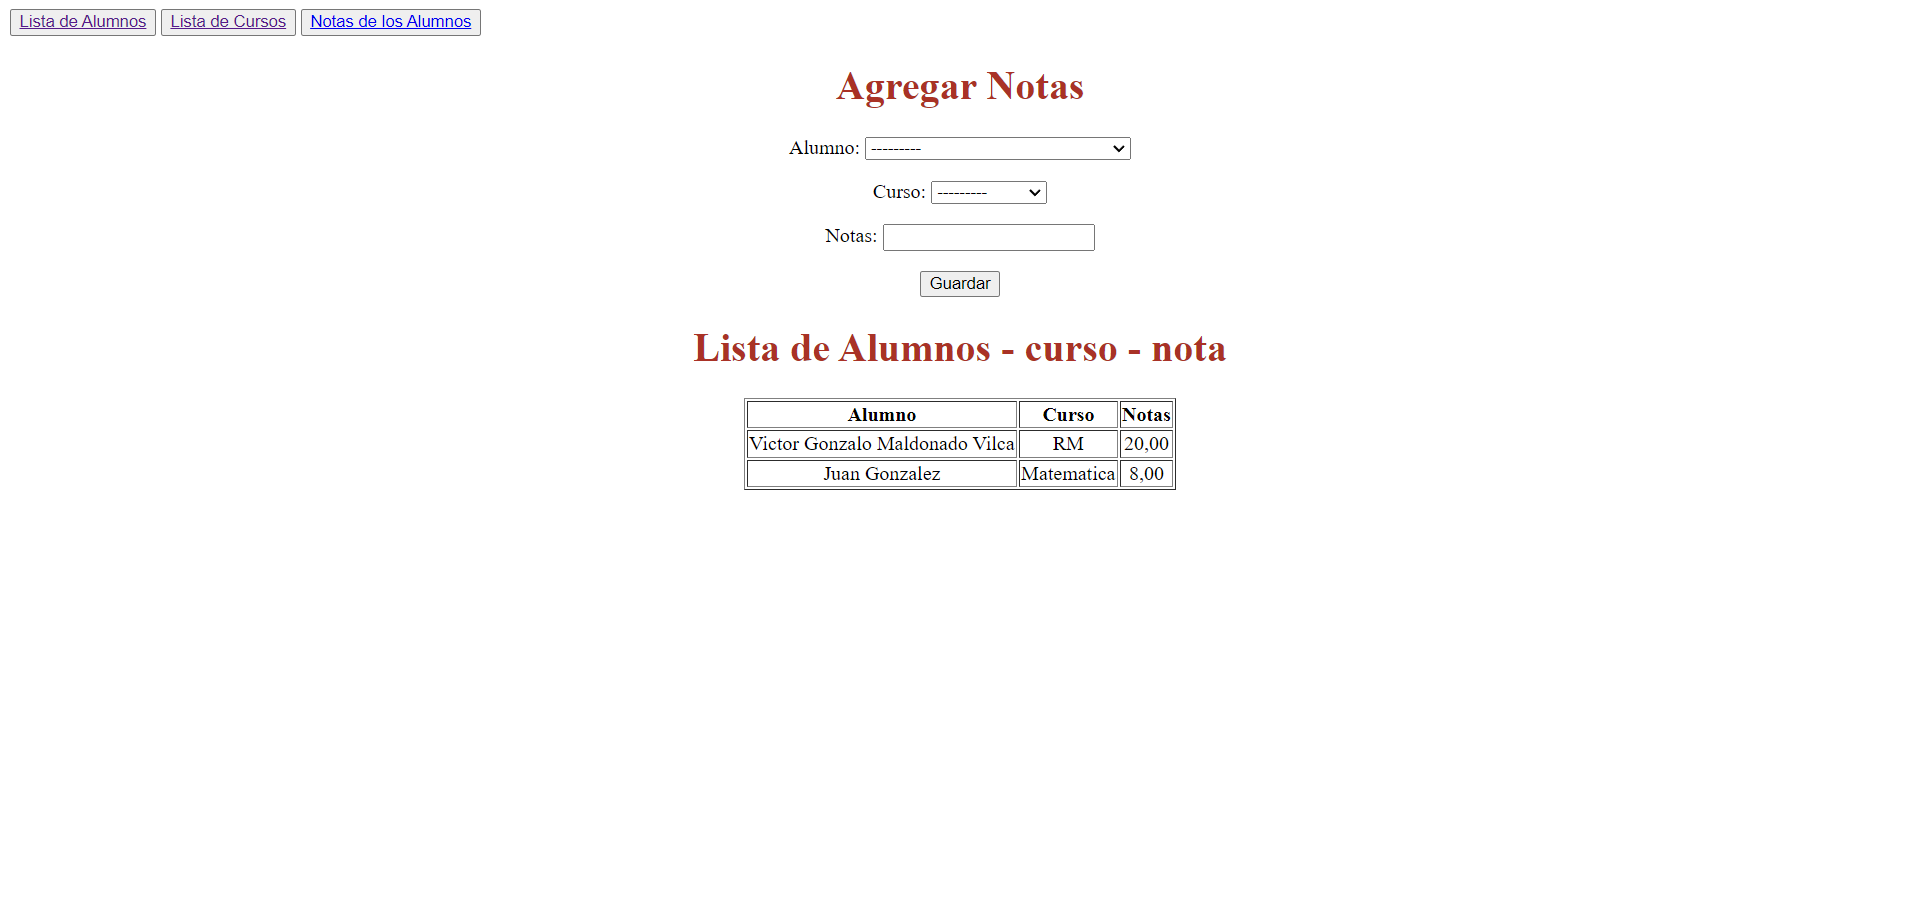
\includegraphics[width=1\textwidth, keepaspectratio]{img/html6.png}
      \caption{Agregar Notas}
    \end{figure}
  \end{itemize}

  
%%%%%%%%%%%%%%%%%%%%
	
  \subsection{Uso de GitHub}
  
%%%%%%%%%%%%%%%%%%%%

	\subsubsection{Usuario de GitHub}
  \begin{figure}[H]
    \centering
    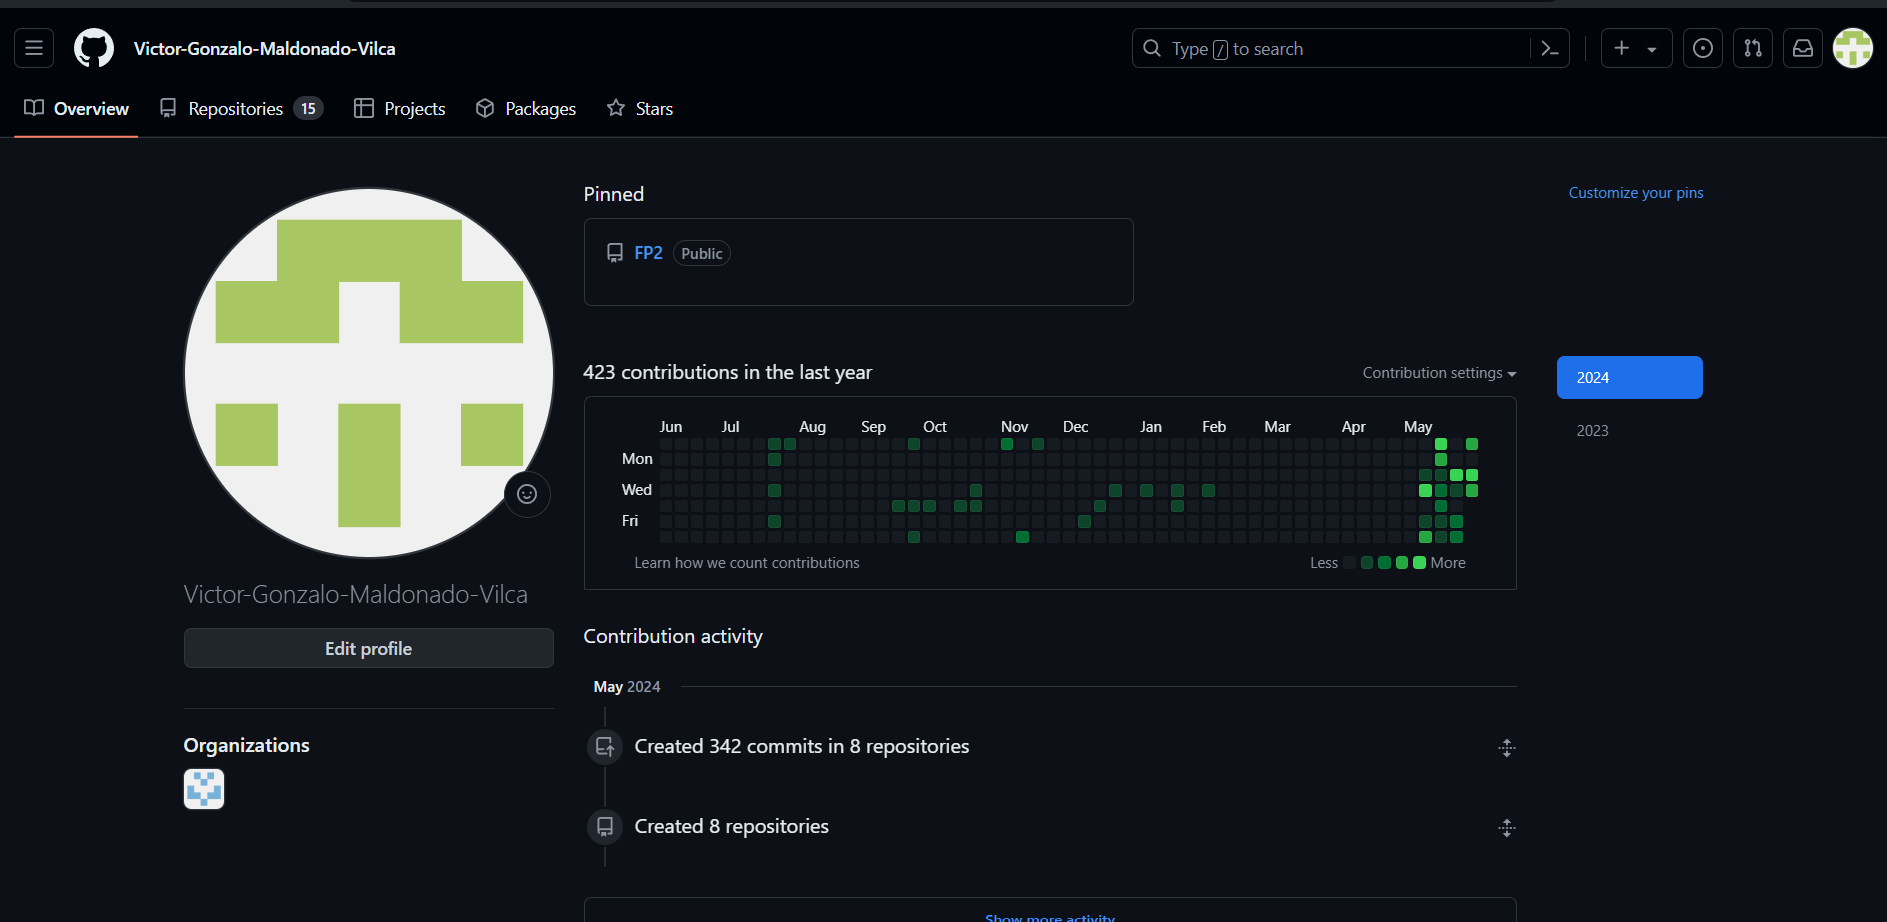
\includegraphics[width=1\textwidth, keepaspectratio]{img/usuario.png}
    \caption{Usuario GitHub}
  \end{figure}
  
%%%%%%%%%%%%%%%%%%%%

  \subsubsection{Creación de un Nuevo Repositorio}
  \begin{figure}[H]
    \centering
    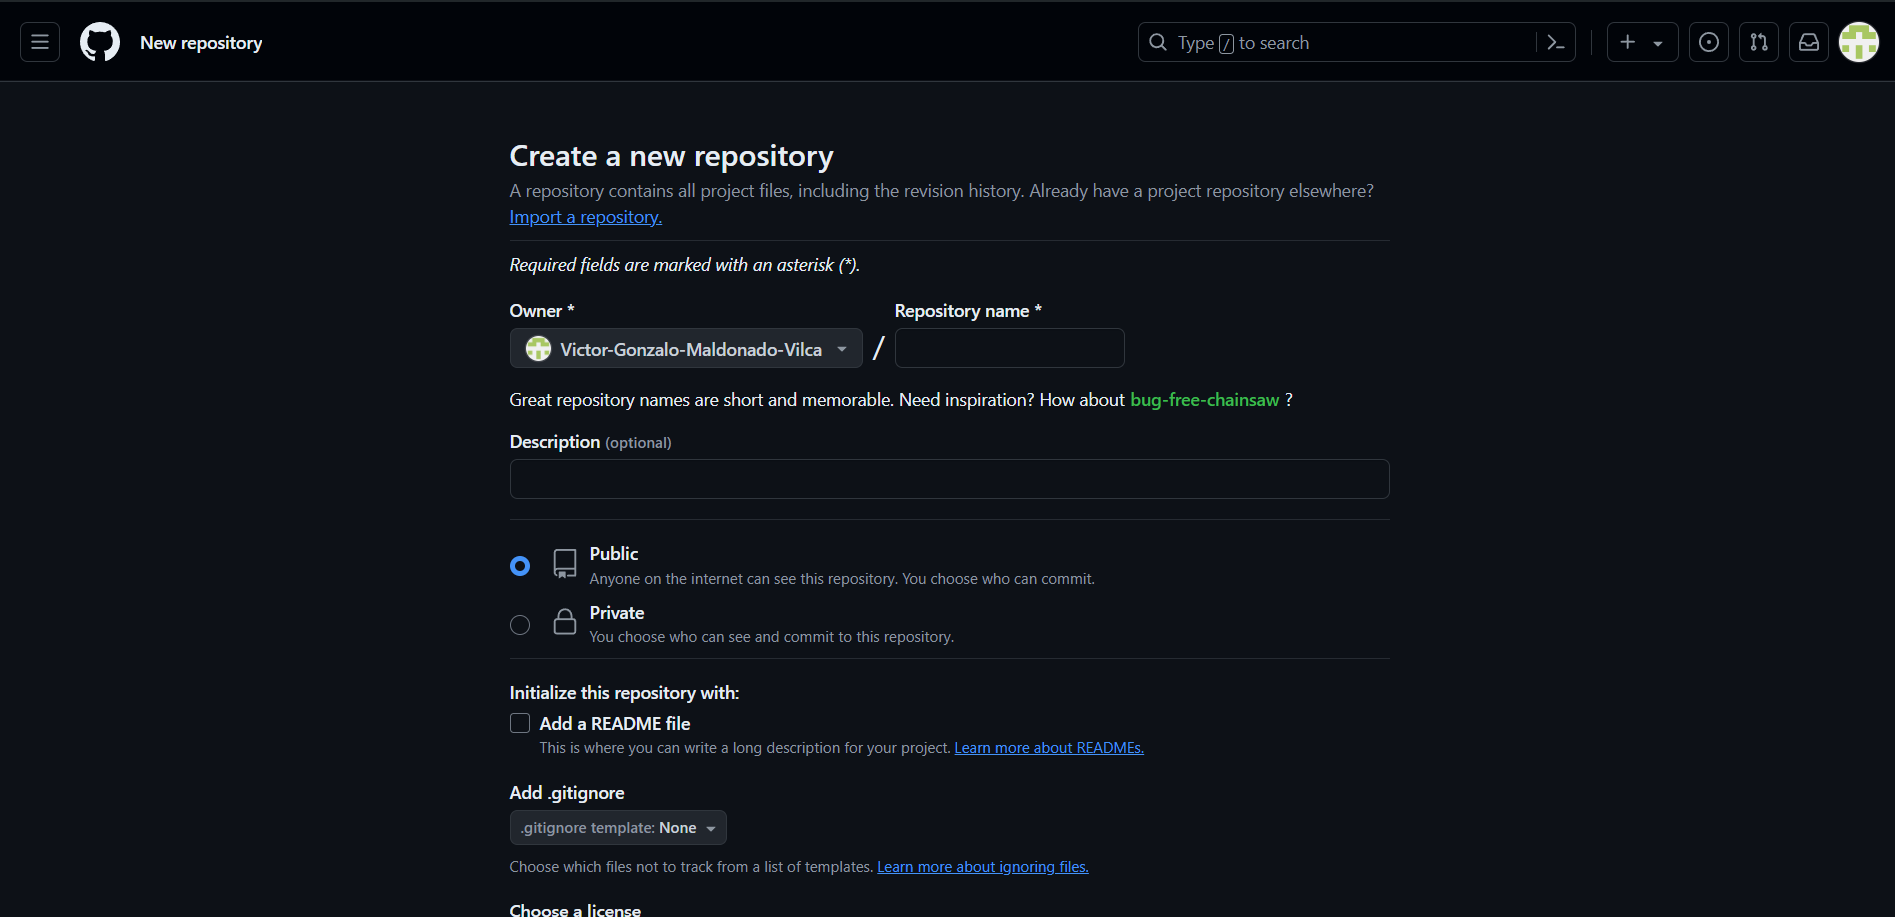
\includegraphics[width=1\textwidth, keepaspectratio]{img/CrearRepo.png}
    \caption{Creación Repositorio}
  \end{figure}
  \newpage
  
%%%%%%%%%%%%%%%%%%%%
	
  \subsubsection{Comandos de Configuración}
  \begin{lstlisting}[language=, caption={Servidor}]
  echo "# lab06" >> README.md
  git init
  git add README.md
  git commit -m "first commit"
  git branch -M master
  git remote add origin https://github.com/Victor-Gonzalo-Maldonado-Vilca/Lab06_Django.git
  git push -u origin master
  \end{lstlisting}
  
%%%%%%%%%%%%%%%%%%%%  
  
  \subsubsection{Implementación de Readme.md}
  \begin{figure}[H]
    \centering
    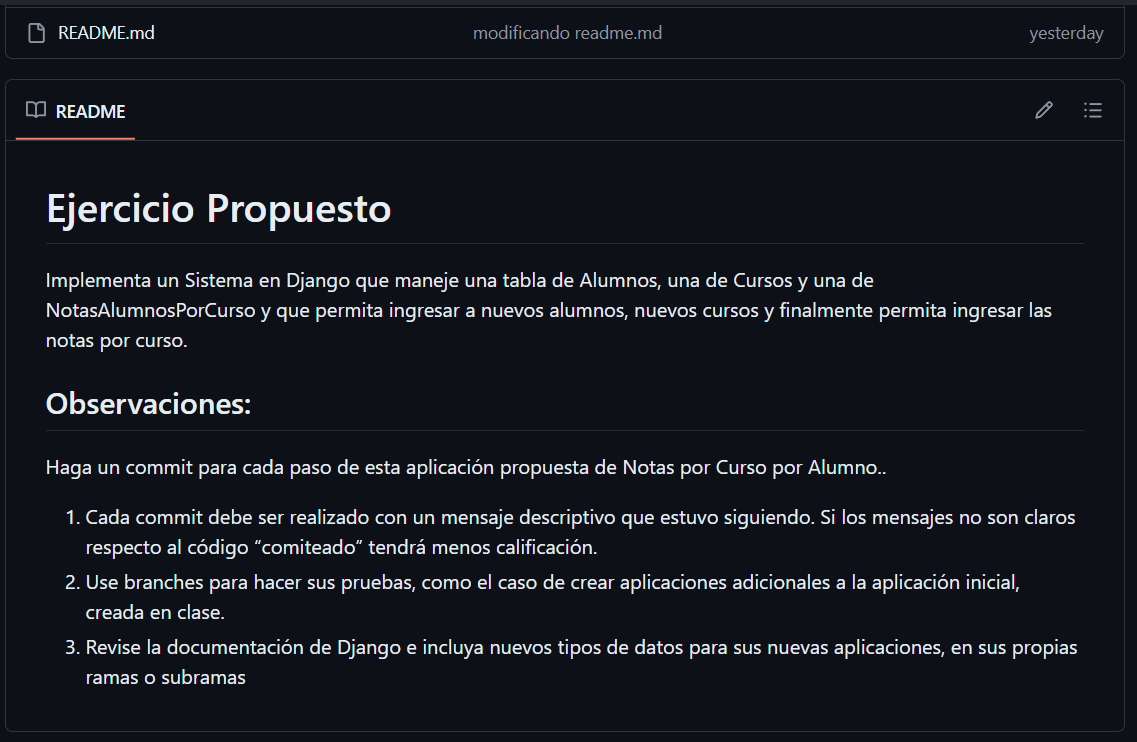
\includegraphics[width=1\textwidth, keepaspectratio]{img/readme.png}
    \caption{Readme.md}
  \end{figure}
  
%%%%%%%%%%%%%%%%%%%%

	\subsubsection{Registro de cambios en mi código}
  \begin{figure}[H]
    \centering
    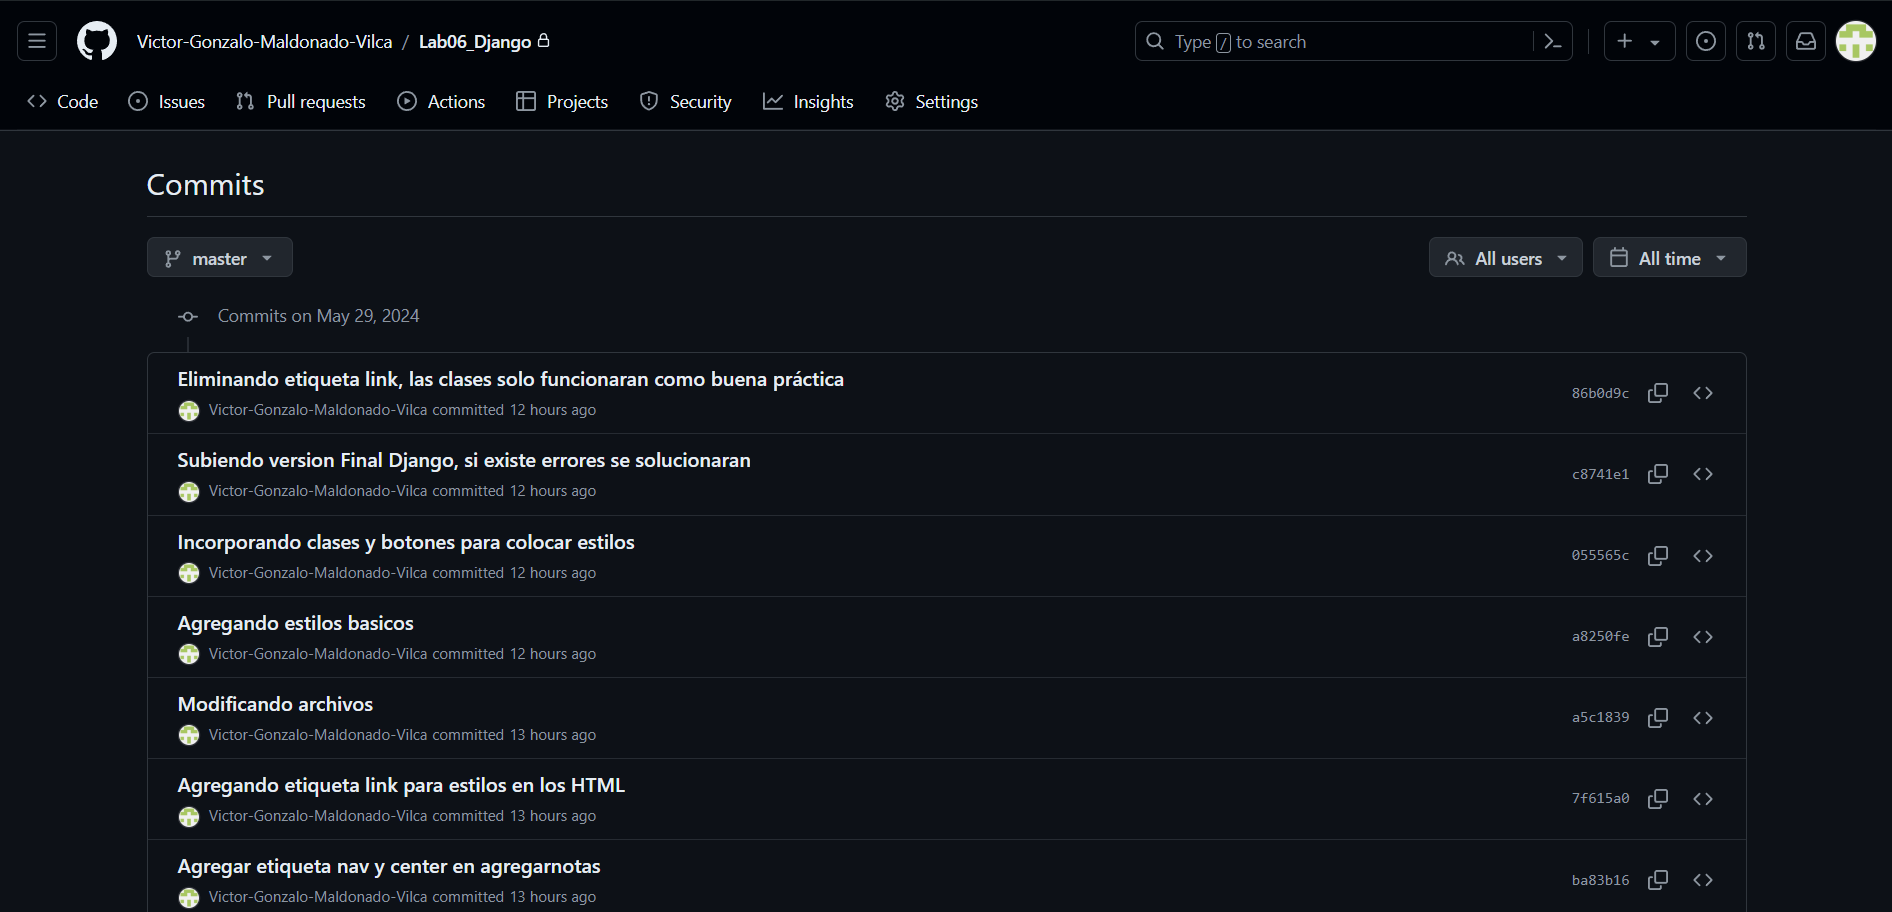
\includegraphics[width=1\textwidth, keepaspectratio]{img/commits.png}
    \caption{Commits}
  \end{figure}
	
%%%%%%%%%%%%%%%%%%%%

	\subsubsection{Repositorio}
  \begin{figure}[H]
    \centering
    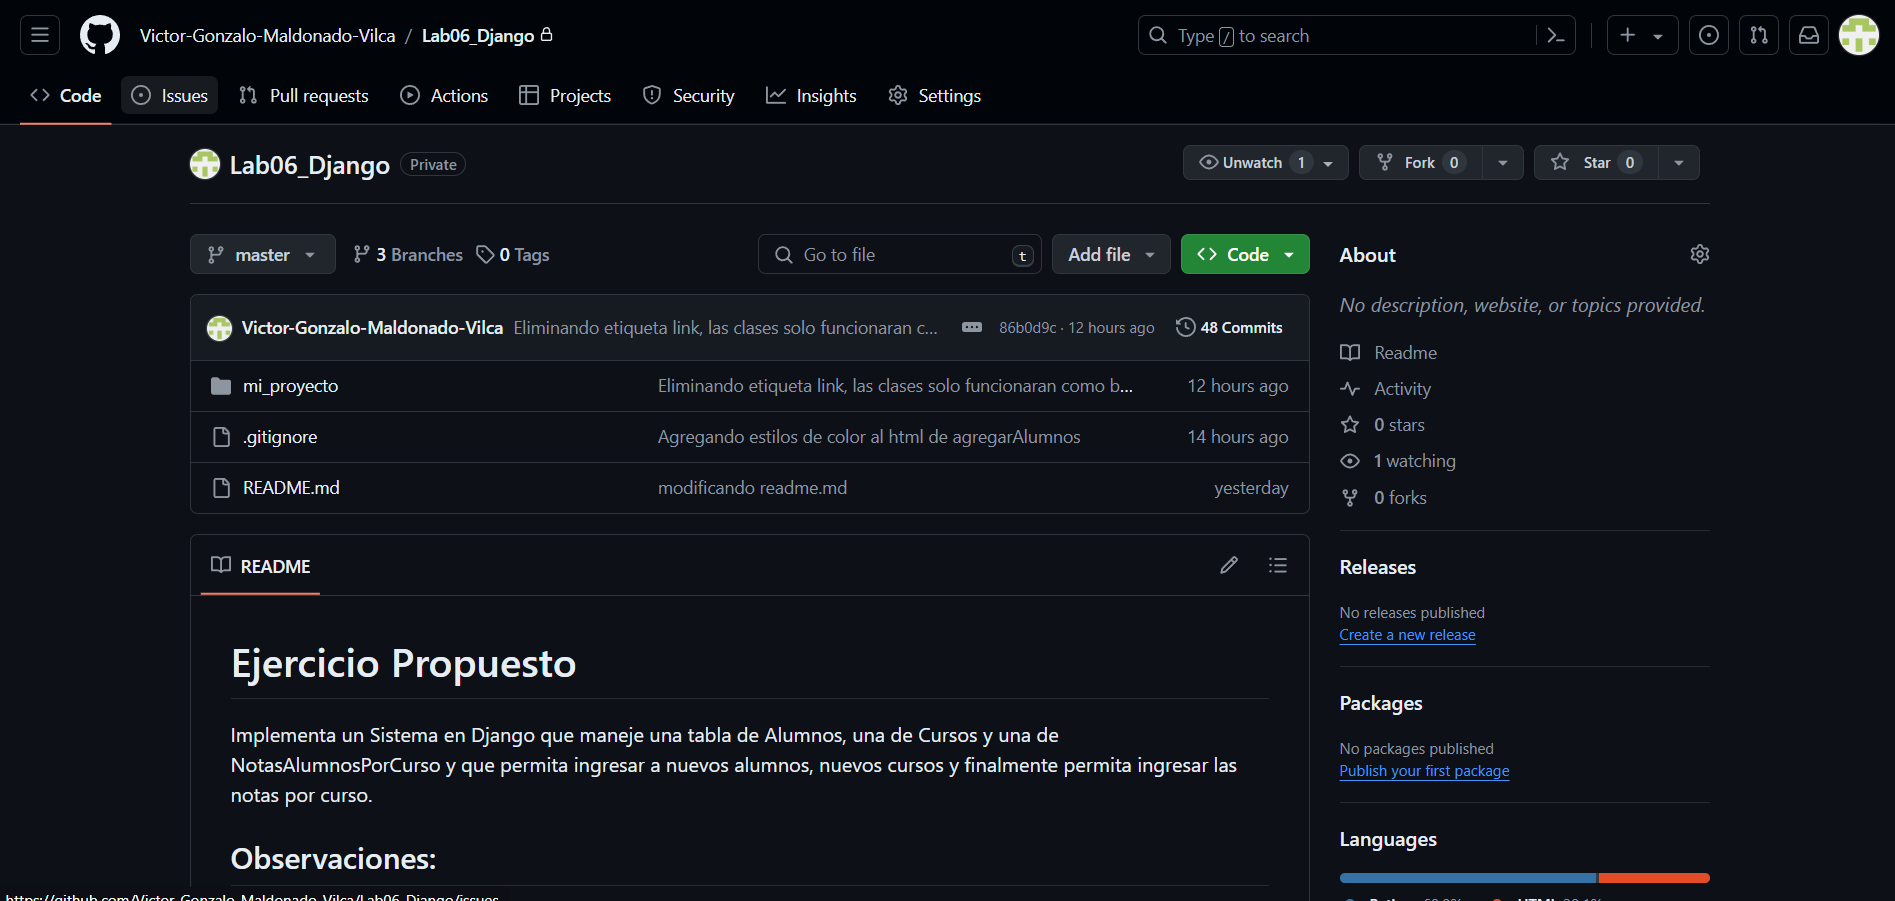
\includegraphics[width=1\textwidth, keepaspectratio]{img/repositorio.png}
    \caption{Repositorio}
  \end{figure}
  
%%%%%%%%%%%%%%%%%%%%
  
\subsubsection{Uso de Ramas}
  \begin{figure}[H]
    \centering
    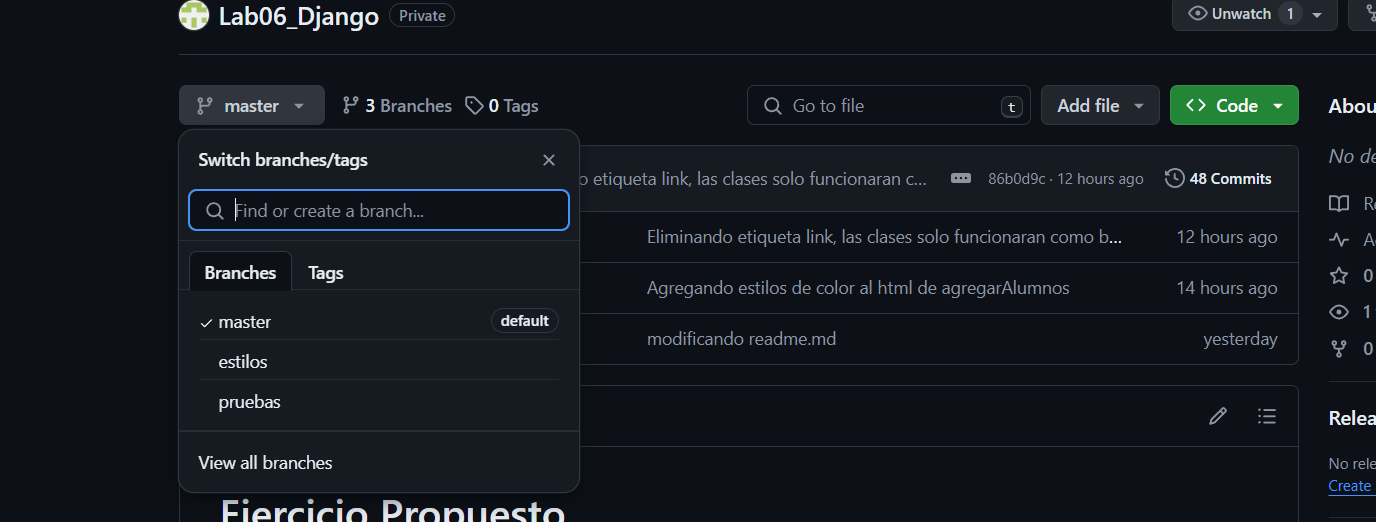
\includegraphics[width=1\textwidth, keepaspectratio]{img/ramas.png}
    \caption{Ramas}
  \end{figure}
  
%%%%%%%%%%%%%%%%%%%%

	\subsubsection{Proyecto compartido con el profesor de github}
  \begin{figure}[H]
    \centering
    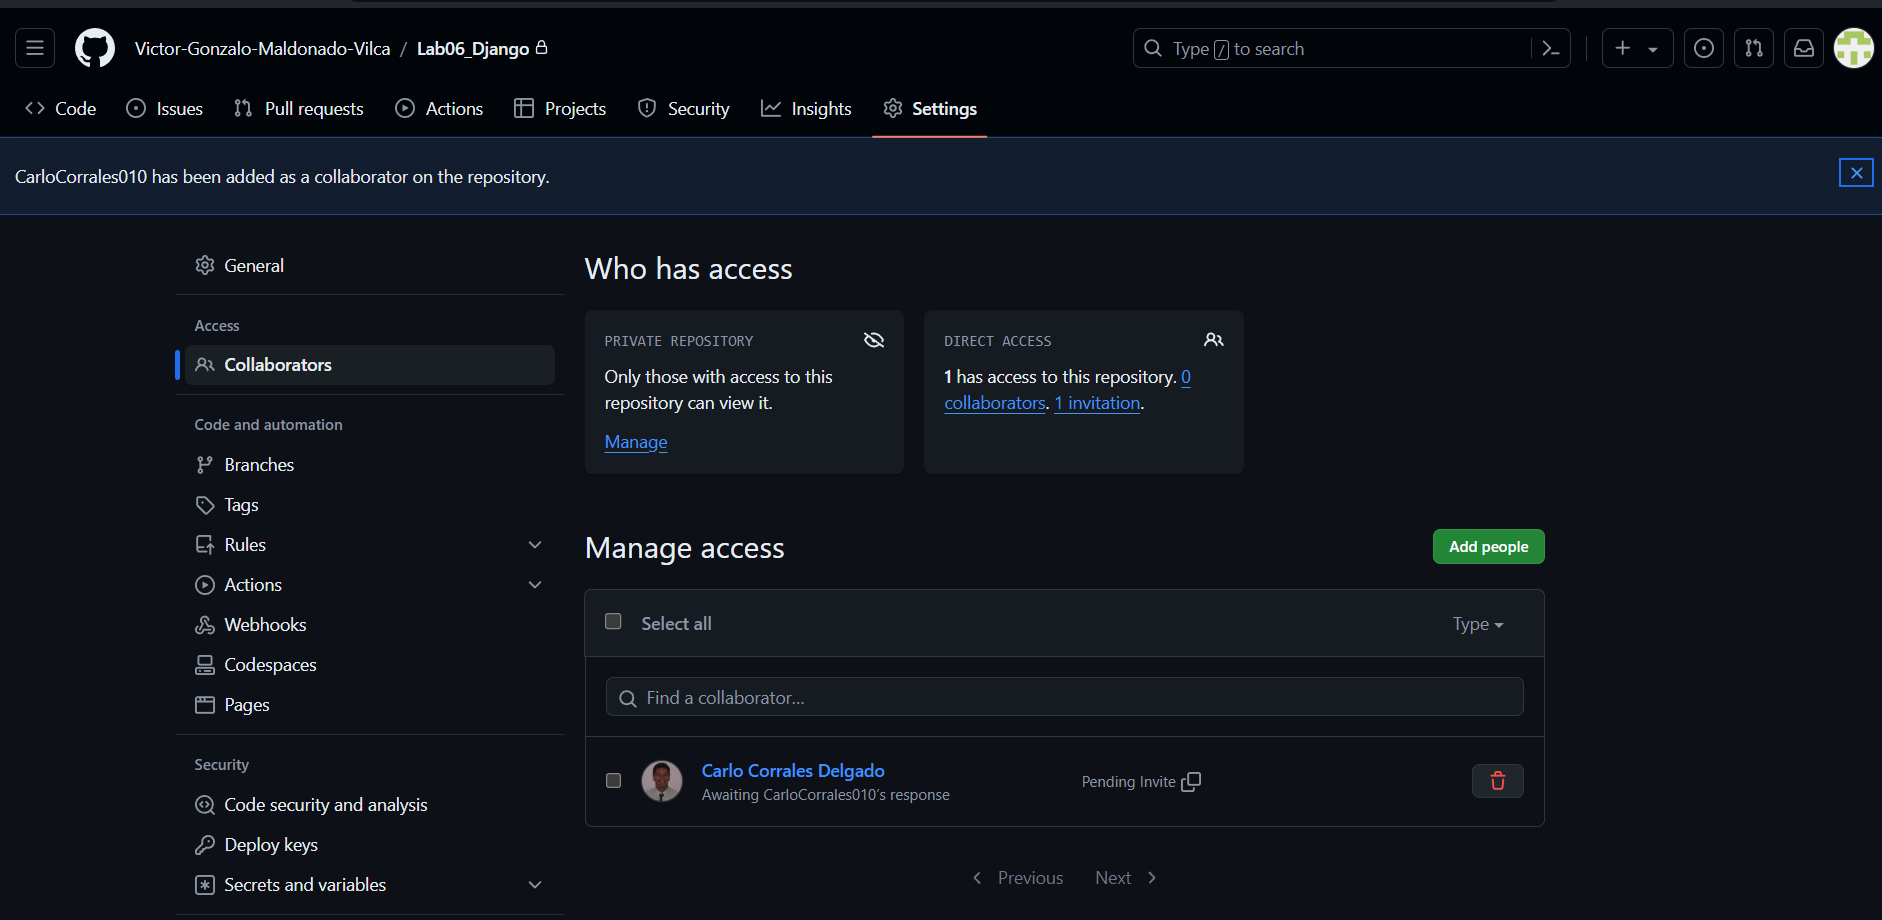
\includegraphics[width=1\textwidth, keepaspectratio]{img/compartir.png}
    \caption{Compartir con el Docente}
  \end{figure}
  \newpage
  
%%%%%%%%%%%%%%%%%%%%

  \section{Recomensaciones}
  \begin{itemize}
    \item Seguir las mejores prácticas de desarrollo de Django, como la separación de la lógica de negocios en vistas y 
    la creación de plantillas reutilizables.
    \item Realizar pruebas unitarias y de integración para garantizar la calidad del código, y asegúrate de implementar 
    medidas de seguridad en tu aplicación.
  \end{itemize}

%%%%%%%%%%%%%%%%%%%%

  \section{Conclusiones}
  \begin{itemize}
    \item Django es un framework web potente y versátil que permite desarrollar aplicaciones web de manera rápida y eficiente.
    \item La arquitectura MVC (Modelo-Vista-Controlador) de Django ayuda a organizar el código de manera estructurada y modular, 
    lo que facilita la mantenibilidad y escalabilidad de las aplicaciones.
    \item Con un buen entendimiento de Django y siguiendo las mejores prácticas de desarrollo, se pueden crear aplicaciones web 
    robustas y de alto rendimiento.
  \end{itemize}

%%%%%%%%%%%%%%%%%%%%
	\newpage
	\subsection{\textcolor{red}{Rúbrica para el contenido del Informe y demostración}}
	\begin{itemize}			
		\item El alumno debe marcar o dejar en blanco en celdas de la columna \textbf{Checklist} si cumplio con el ítem correspondiente.
		\item Si un alumno supera la fecha de entrega,  su calificación será sobre la nota mínima aprobada, siempre y cuando cumpla con todos lo items.
		\item El alumno debe autocalificarse en la columna \textbf{Estudiante} de acuerdo a la siguiente tabla:
	
		\begin{table}[ht]
			\caption{Niveles de desempeño}
			\begin{center}
			\begin{tabular}{ccccc}
    			\hline
    			 & \multicolumn{4}{c}{Nivel}\\
    			\cline{1-5}
    			\textbf{Puntos} & Insatisfactorio 25\%& En Proceso 50\% & Satisfactorio 75\% & Sobresaliente 100\%\\
    			\textbf{2.0}&0.5&1.0&1.5&2.0\\
    			\textbf{4.0}&1.0&2.0&3.0&4.0\\
    		\hline
			\end{tabular}
		\end{center}
	\end{table}	
	

	\end{itemize}

 
	
	\begin{table}[H]
		\caption{Rúbrica para contenido del Informe y demostración}
		\setlength{\tabcolsep}{0.5em} % for the horizontal padding
		{\renewcommand{\arraystretch}{1.5}% for the vertical padding
		%\begin{center}
		\begin{tabular}{|p{2.7cm}|p{7cm}|x{1.3cm}|p{1.2cm}|p{1.5cm}|p{1.1cm}|}
			\hline
    		\multicolumn{2}{|c|}{Contenido y demostración} & Puntos & Checklist & Estudiante & Profesor\\
			\hline
			\textbf{1. GitHub} & Hay enlace URL activo del directorio para el  laboratorio hacia su repositorio GitHub con código fuente terminado y fácil de revisar. &2 &X &2 & \\ 
			\hline
			\textbf{2. Commits} &  Hay capturas de pantalla de los commits más importantes con sus explicaciones detalladas. (El profesor puede preguntar para refrendar calificación). &4 &X &4 & \\ 
			\hline 
			\textbf{3. Código fuente} &  Hay porciones de código fuente importantes con numeración y explicaciones detalladas de sus funciones. &2 &X &2 & \\ 
			\hline 
			\textbf{4. Ejecución} & Se incluyen ejecuciones/pruebas del código fuente  explicadas gradualmente. &2 &X &2 & \\ 
			\hline			
			\textbf{5. Pregunta} & Se responde con completitud a la pregunta formulada en la tarea.  (El profesor puede preguntar para refrendar calificación).  &2 &X &2 & \\ 
			\hline	
			\textbf{6. Fechas} & Las fechas de modificación del código fuente estan dentro de los plazos de fecha de entrega establecidos. &2 &X &2 & \\ 
			\hline 
			\textbf{7. Ortografía} & El documento no muestra errores ortográficos. &2 &X &2 & \\ 
			\hline 
			\textbf{8. Madurez} & El Informe muestra de manera general una evolución de la madurez del código fuente,  explicaciones puntuales pero precisas y un acabado impecable.   (El profesor puede preguntar para refrendar calificación).  &4 &X &4 & \\ 
			\hline
			\multicolumn{2}{|c|}{\textbf{Total}} &20 & &20 & \\ 
			\hline
		\end{tabular}
		%\end{center}
		%\label{tab:multicol}
		}
	\end{table}


%%%%%%%%%%%%%%%%%%%%%%%%%%%%%%%%%%%%%%%%%%%%%%%%%%%%%%%%%%%%%%%%%%%
	
  \newpage
  \section{Referencias}
  \begin{itemize}
    \item \url{https://docs.djangoproject.com/en/5.0/}
    \item \url{https://docs.github.com/es}
    \item \url{https://git-scm.com/doc}
  \end{itemize}

%%%%%%%%%%%%%%%%%%%% 
%\clearpage
%\bibliographystyle{apalike}
%\bibliographystyle{IEEEtranN}
%\bibliography{bibliography}
			
\end{document}
